\chapter{{\em Silhouette} Execution}
In the previous two chapters,
we have identified how and why
multiple executions of the same
Linux service can diverge in behavior.
In light of our results, this chapter introduces a 
novel design strategy that aims to mitigate the bootstorm problem:
{\em silhouette} execution (Section \ref{def:sil}).
It also describes the simple simulation techniques we used 
to model the effectiveness of silhouette
execution in reducing CPU pressure for concurrently booting VMs 
(Section \ref{silsimulation}).
From the results of our simulations, we present design ideas
that can improve the effectiveness of
silhouette execution (Section \ref{silimprove})
and evaluate them (Section \ref{sileval}).
Our simulations show that the proposed designs can be successful
in mitigating the bootstorm problem. 

\section{What is {\em Silhouette} execution?} \label{def:sil}
The previous few chapters showed that
distinct executions of the same Linux service
generally execute the same number of instructions
across identical VMs. If the number of booting VMs for
the same physical host is large (as is 
the case in VDI deployments),
then executing many instructions over
and over again during boot represents a waste of scarce CPU cycles.
{\em Silhouette} execution, in essence, targets
redundant execution of the same instructions across different
instances in order to reduce CPU pressure in bootstorm
scenarios. As illustrated by Figure \ref{silconcept},
this approach can extend host CPU capabilities much like
memory overcommitment extends
the host memory resources.

\begin{figure}
  \centering
  
\includegraphics[scale=0.64, trim=1cm 0cm 1cm 0cm]{none.jpg}
  \caption[Silhouette execution is to the CPU what memory overcommitment
    is to the memory subsystem.]%
          {Silhouette execution is to the CPU what memory overcommitment
          is to the memory subsystem.}
  \label{silconcept}
\end{figure}

Broadly speaking, {\em silhouette} execution captures the
novel design idea that information recorded from one
execution of a program -- the {\em leader} -- can be used to 
bypass execution steps of subsequent instances
of the same program -- the {\em silhouettes}. 
Ideally, the leader executes all instructions from the program, 
while the silhouettes execute a significantly smaller subset
of these instructions. To maintain correctness,
silhouettes need only execute: 

\begin{itemize}
\item instructions that can potentially cause the leader's
  execution to differ from the silhouettes (e.g. the \texttt{rdtsc}
  instruction); 
\item instructions that propagate any earlier differences in execution; 
\item instructions that read or write to memory;
\item system calls that have side-effects to external entities
  from the operating system (e.g. the \texttt{read} system 
  call mutates operating system state associated with file descriptors).
  
\end{itemize}

Ideally, if there are no differences between the leader's
execution and a silhouette's, then the silhouette would only
execute the system calls or load/store instructions
executed by the leader until the login screen is shown.
Assuming that the leader and a silhouette start from the same
memory image, executing all the loads and stores
ensures that the memory image of the two instances
are identical at the end. Executing all the system
calls with the same arguments also ensures
that the silhouette's execution is {\em faithful}
to its semantics i.e. the side-effects to the underlying
operating system are maintained at the end.
When the number of system calls and memory read/writes
are much less than all instructions executed,
this approach can, in theory, reduce the stress
placed on the host CPU.

Precise knowledge of where program execution can diverge 
is indispensable to getting silhouette execution
to work, because instructions that can 
diverge execution need to be dynamically identified.
Our detailed analysis of the various interfaces
between application programs and the operating system
allows us to identify such potential sources of
execution divergence.

The fundamental difference
between silhouette execution and record-and-replay
approaches is that silhouette execution
does not semantically alter subsequent executions
of a program by emulating the leader's execution. 
Conceptually, silhouettes are independent executions of a program
that can potentially branch from the leader's execution at any point
because we execute all system calls on behalf of silhouettes.

The next few subsections outline a few
designs that employ silhouette execution
on individual user-space programs
running on concurrently booting VMs.
These designs can be further generalized to the execution of entire
VMs themselves; this would require us to precisely
identify the nondeterminism that can
arise from all software layers inside a VM.
We focus using silhouette execution for user-space programs as 
a first step to solving the bootstorm problem: after all, as outlined
Section \ref{linuxboot}, booting VMs
can saturate host CPUs when they launch many
identical user-space processes.

\subsection{{\em Precise Silhouetting}}\label{precise:sil}
Here is a simple design that uses silhouette execution 
to reduce CPU overhead in the bootstorm scenario: 

\begin{enumerate}

\item We run one program instance -- the {\em leader} -- 
slightly ahead of all other program instances -- the {\em silhouettes}.

\newpage
\item Using dynamic instrumentation techniques on the leader, we
\begin{itemize}
\item precisely identify instructions where other instances of the
program could {\em potentially} diverge. We call these instructions {\em fork-points}.
\item collect an {\em execution signature} that summarizes the 
leader's execution between successive fork-points. For a user-space program, 
this includes a record of memory operations and 
deterministic system calls.
\end{itemize}

\item When a leader reaches a fork-point, it sends its
own execution signature from the previous fork-point (or the
beginning of the program) till the current fork-point to all
other silhouettes. It then waits for all silhouettes
to catch up in execution and reach the fork-point as well.

\item The silhouettes do not execute
all the instructions that the leader executes.
Instead, each silhouette bypasses execution between
two fork-points by executing only the memory
operations and system calls from the 
execution signature sent by the leader,
and restoring the register state at the end.

\item 
When the leader and the silhouettes
have caught up, they execute the {\em forking} instruction
in sync and observe its side-effects.
The forking instruction may or 
may not behave differently
in a silhouette than the leader.

\begin{itemize}
\item If the forking instruction
does have different side-effects
in a silhouette, the silhouette branches execution and 
executes instructions independently
from that point onwards. 

\item Otherwise, we
return to Step 2: the leader
executes instructions till
the next fork-point (or the desired
end-point) while the silhouettes 
wait for the next execution signature.
\end{itemize}
\end{enumerate}

\noindent We name this design {\em precise silhouetting} because
it cannot tolerate any differences in execution
between the multiple instances of a program:
silhouettes completely branch
execution after executing a
forking instruction that disagrees
with the leader. 

Our description of precise silhouetting requires
that the leader executes concurrently
with the silhouettes -- albeit slightly ahead --
but this is not necessary.
This approach would work even
if we run the leader to completion
before we run any silhouettes. 
The silhouettes, of course, would only execute system calls and memory
operations between
successive fork-points that the leader recorded earlier.

\subsection{\em Optimistic Silhouetting (excluding control flow)}\label{opt:sil}
{\em Optimistic silhouetting} essentially follows the 
same overall design principles
as precise silhouetting,
except that it allows silhouettes
to tolerate minor execution differences 
before branching execution completely.
In this design:

\begin{enumerate}
\item The leader executes slightly ahead of the silhouettes. 
  The leader identifies fork-points and sends
  execution signatures to silhouettes. 
  The silhouettes bypass execution by only 
  executing the load/store instructions
  and system calls made by the leader.
  This is similar to what happens
  in precise silhouetting.

\item Unlike the previous design, however, if a forking 
instruction has different
side-effects in a silhouette
than the leader,
\begin{itemize}
\item the silhouette does not immediately 
  branch execution completely;
\item the leader tracks the register or 
  memory values that are written differently
  in the multiple instances
  by marking them as {\em tainted}.
  The leader treats any instructions that 
  read tainted values as
  fork-points as well.
\end{itemize}

\item When fork-points 
become too frequent, or when
control flow diverges (e.g. a tainted
value is compared to a constant to
determine control flow),
a silhouette starts
executing instructions independently
and branches off from the leader.
\end{enumerate}

\noindent This approach does require that we
run the leader and its silhouettes
at the same time, with the leader
slightly ahead of the silhouettes.
Concurrent execution significantly reduces
the complexity associated with taint propagation
during the leader's execution,
because the leader would
have to compute
{\em all} possible fork points
ahead of time otherwise.

\subsection{\em Optimistic Silhouetting (including control flow)}\label{opt:sil}
This design is similar in essence to the version of {\em optimistic silhouetting}  
described above, but it can also tolerate minor control flow
differences between the leader and the silhouettes. The leader and the
silhouettes must execute concurrently. In this design:

\begin{enumerate}

\item As before, the leader executes
  slightly ahead of the silhouettes, records
  and transmits execution signatures, and uses dynamic taint propagation 
  to tolerate minor differences in instruction side-effects.

\item Unlike before, the leader uses dynamic instrumentation to
  create a dynamic {\em control flow graph}
  for the program execution as well:
\begin{itemize}
\item  When the leader and a silhouette reach a
  control flow fork-point (e.g. after a tainted value
  is read to determine control flow), the
  leader uses the dynamic control flow
  graph to determine when the {\em immediate post-dominator}
  of the block where execution has diverged.

\item   The silhouette branches off
  temporarily (rather than permanently)
  and executes independently to the 
  point of control flow convergence.
  The silhouette and the leader log
  any memory values written 
  or any system calls made
  during this {\em branch interval}.

\item 
  The leader and the silhouette
  compare their current register state, along with the system calls made
  or memory values written during the branch interval. 
  Any conflicting memory addresses 
  or register values are
  marked by the leader as tainted.
\end{itemize}

\item The leader resumes
  execution as before; the silhouette
  follows a little behind 
  and waits to skip-ahead to the next fork-point.
  When fork-points become too frequent,
  execution branches permanently.

\end{enumerate}

\section{Simulation Scheme} \label{silsimulation}

\subsection{Design Metrics}

Several specific metrics seem important in
evaluating the feasibility of silhouette
execution for the bootstorm scenario:
\begin{itemize}
\item Ideally, delaying the first fork-point
to be as late into silhouette execution as possible
would {\em guarantee} that we avoid
executing many redundant instructions and
save on CPU usage.
\item More generally, having few
fork-points is desirable because it reduces
the design complexity and overhead associated with 
figuring out whether a silhouette has diverged
in execution from a leader or not.
\item Having fork-points that are
separated by very many instructions
can help compress execution logs.
For instance, we could forget intermediate
values of memory locations and only
remember their final values instead.
\item Finally, programs that have a high
ratio of user-mode instructions to system-calls
and memory operations would clearly 
improve the savings from silhouette execution.
\end{itemize}


We modified our data collection scheme from Chapter \ref{ch:boot} (shown in 
Figure \ref{data:naive}) to simulate and
evaluate silhouette execution in the bootstorm scenario.

\begin{figure}[]
  \center
  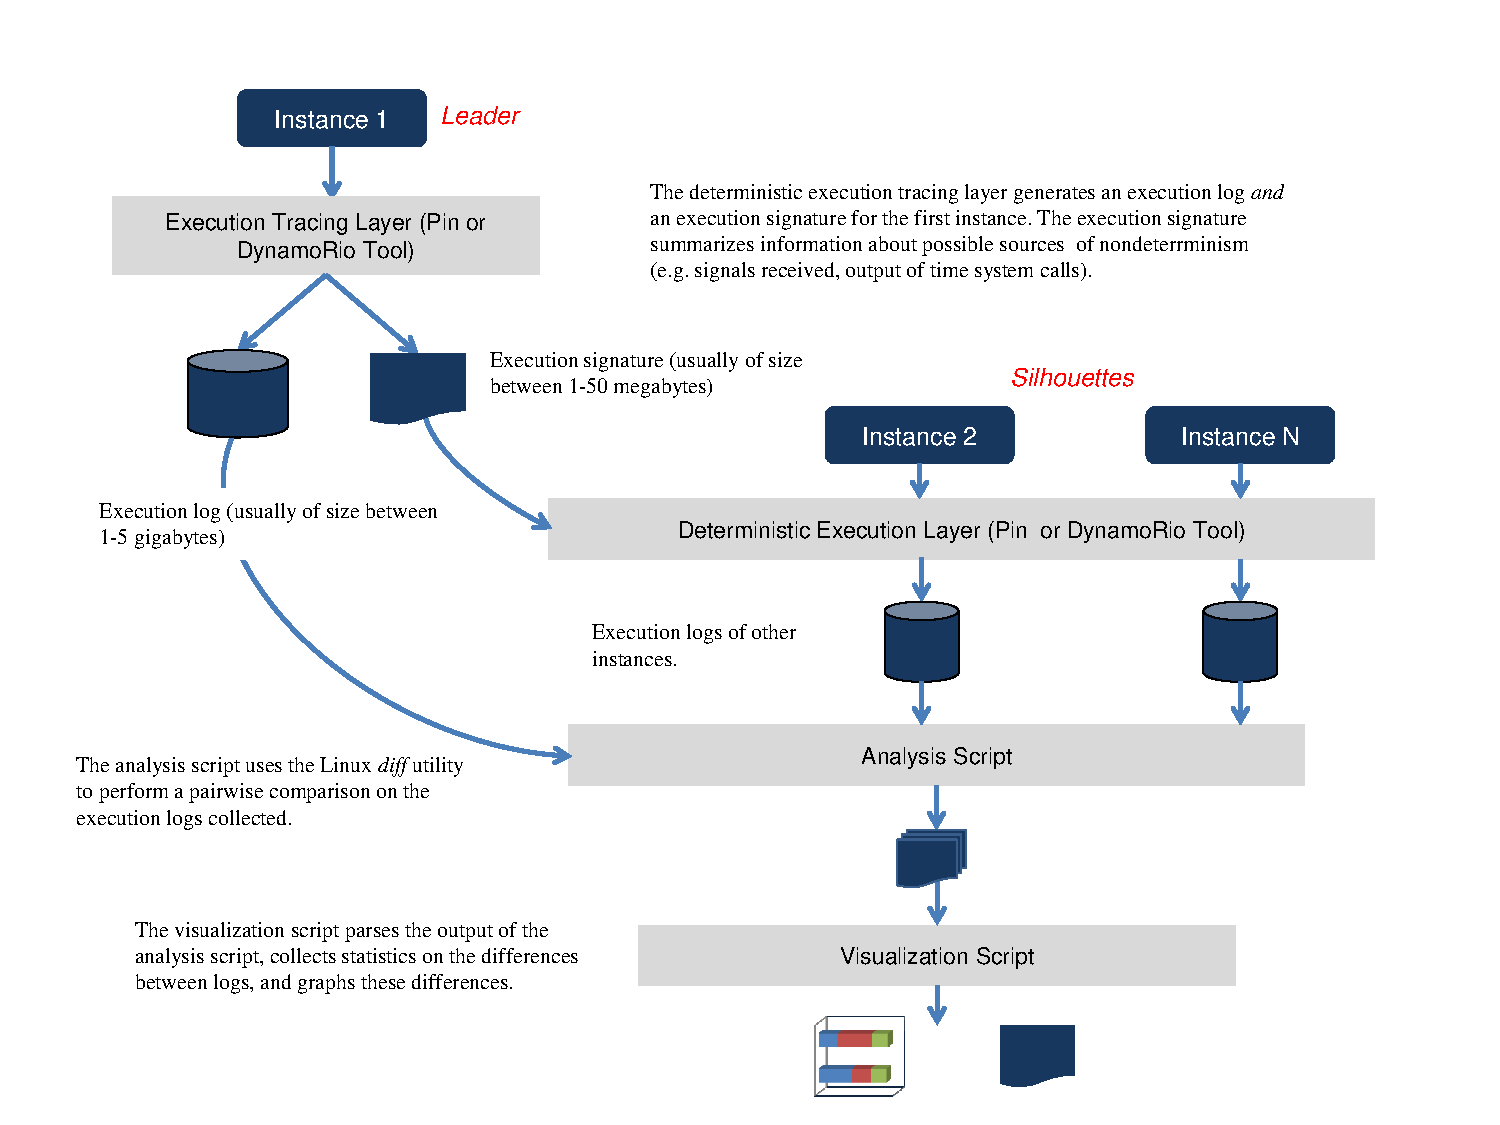
\includegraphics[scale=0.7, trim=1cm 0cm 1cm 0cm]
                  {simulation.pdf}
  \caption[Simulation of {\em Silhouette Execution} in a bootstorm scenario]%
  {Simulation of {\em Silhouette Execution} in a bootstorm scenario.
    We use dynamic instrumentation to 
    generate an execution signature file for the leader.
    While we do not bypass execution in the 
    silhouettes, try to reduce the number of fork-points 
    and record information about them.
    Our analysis and visualization
    scripts allow us to simualate and evaluate
    the effectiveness of {\em silhouette} execution.
  }
  \label{ch3:figsimulation}
\end{figure}

As shown by Figure \ref{ch3:figsimulation}, we run one instance of the
program -- the {\em leader} -- before all others.
For the leader, we generate an {\em execution log}, as before,
but we also augment the log by summarizing information about the sources of nondeterminism
described in Section \ref{ch3:sources}. For instance, we record
information about signal timing, process IDs, time-related system calls
in the {\em execution signature} file. Our dynamic instrumentation tool
uses the execution signature of the leader
to modify the instruction sequences executed by subsequently
executions (the {\em followers}), to boost determinism as much as possible.
Even though we use specific terminology, this simulation scheme can be
reconciled with multiple possible solutions to the 
boot storm scenario that involve:
\begin{itemize}
\item
booting one VM before others,
then using its execution trace to {\em speed-boot} other VMs
in a less hardware-intensive manner, or
\item 
running VMs concurrently but with an assigned leader;
the VMs communicate with each other to overcome
nondeterminism.
\end{itemize}

In the first case, the execution signature file
conceptually represents the trace of the first VM used to speed-boot
other VMs. In the second case, it represents a log of the communications 
sent from the leader sent to concurrently booting VMs. Possible
design ideas for the bootstorm scenario are described 
in Chapter \ref{ch:design}.

\section{Improving Silhouette Execution} \label{silimprove}
We now briefly describe how dynamic instrumentation can be used to overcome
the sources of nondeterminism described in \ref{ch3:sources}. \newline

\noindent {\bf Address Space Layout Randomization (ASLR)} \newline
Existing record-and-replay systems get around ASLR by
forcing the operating system to use the same address space layout across
different runs. A slightly more complex approach 
would use base/offset computations to translate two equivalent 
addresses between different executions. 
For our experiments, we simply disabled ASLR using the command
\texttt {sudo kernel.randomize\_va\_space=0} to simulate the 
case where we nudge the operating system to construct
similar address spaces for the same process. \newline

\noindent {\bf Canary and Pointer Guard Values} \newline
Dynamic instrumentation can be used to force canary (\texttt{gs:0x14})
and pointer guard (\texttt{gs:0x18}) values
to agree across distinct executions of the same program:
instructions that initialize them can be
modified or replaced; the \texttt{AT\_RANDOM} bytes 
provided by the kernel can be
modified before they are read by the application; 
values read from \texttt{`/dev/urandom'} can be 
intercepted and modified; the \texttt{rdtsc} instruction can be emulated.
The last three approaches are needed to control nondeterminism
from randomization anyway and suffice for our purpose. \newline

\noindent {\bf Randomization and Time} \newline
To overcome nondeterminism resulting from randomization,
we need to intercept the standard techniques
used by programs to seed PRNGs.
As already mentioned, values read from \texttt{`/dev/urandom'}
or the \texttt{rdtsc} instruction can be easily replaced
using the execution signature file for the first instance.

Time-related system calls can
be intercepted in the same manner:
the timestamps logged
in the execution signature file
can be used to force agreement
between different executions.
For most time-related system calls,
high-fidelity replay is not necessary:
several timestamps generated
during program execution are simply ignored
(e.g. from \texttt{stat} calls),
so they can actually be replaced with any 
fixed value. Many timestamps
returned from system calls are only compared to
determine ``freshness'': they
can be replaced with deterministic ordinal values (e.g 0 or 1) that 
perserve the original comparison result.

Conceptually, these approaches simulate the possible but highly
unlikely case that all the instances of the same program
executed time-related system calls
at precisely the same times,
and several randomly generated values independently agreed. \newline

\noindent {\bf Signal Delivery} \newline
In order to overcome the unpredictable timing and 
order of signals, we intercept all signals received by 
an application and ensure they are delivered
at precisely the same instruction counts
and in the same order as that indicated
in the execution signature file.

Unlike record-and-replay systems, we only
deliver signals that are {\em actually}
received. Thus, signals that are received earlier
than expected are simply delayed or reordered. If,
however, a signal is not received at the expected
instruction count, our instrumentation tool
simply waits or inserts \texttt{nops} until the 
desired signal is received. If a signal simply
refuses to appear for a long time, execution
must diverge. In our experiments,
this final case does not occur as long
as other sources of nondeterminism are controlled. \newline

\noindent {\bf Process IDs} \newline
Nondeterminism from process IDs
can be controlled by virtualizing the process ID
layer, as shown by Figure \ref{ch3:pidfig}.

\begin{figure}[h]
  \center
  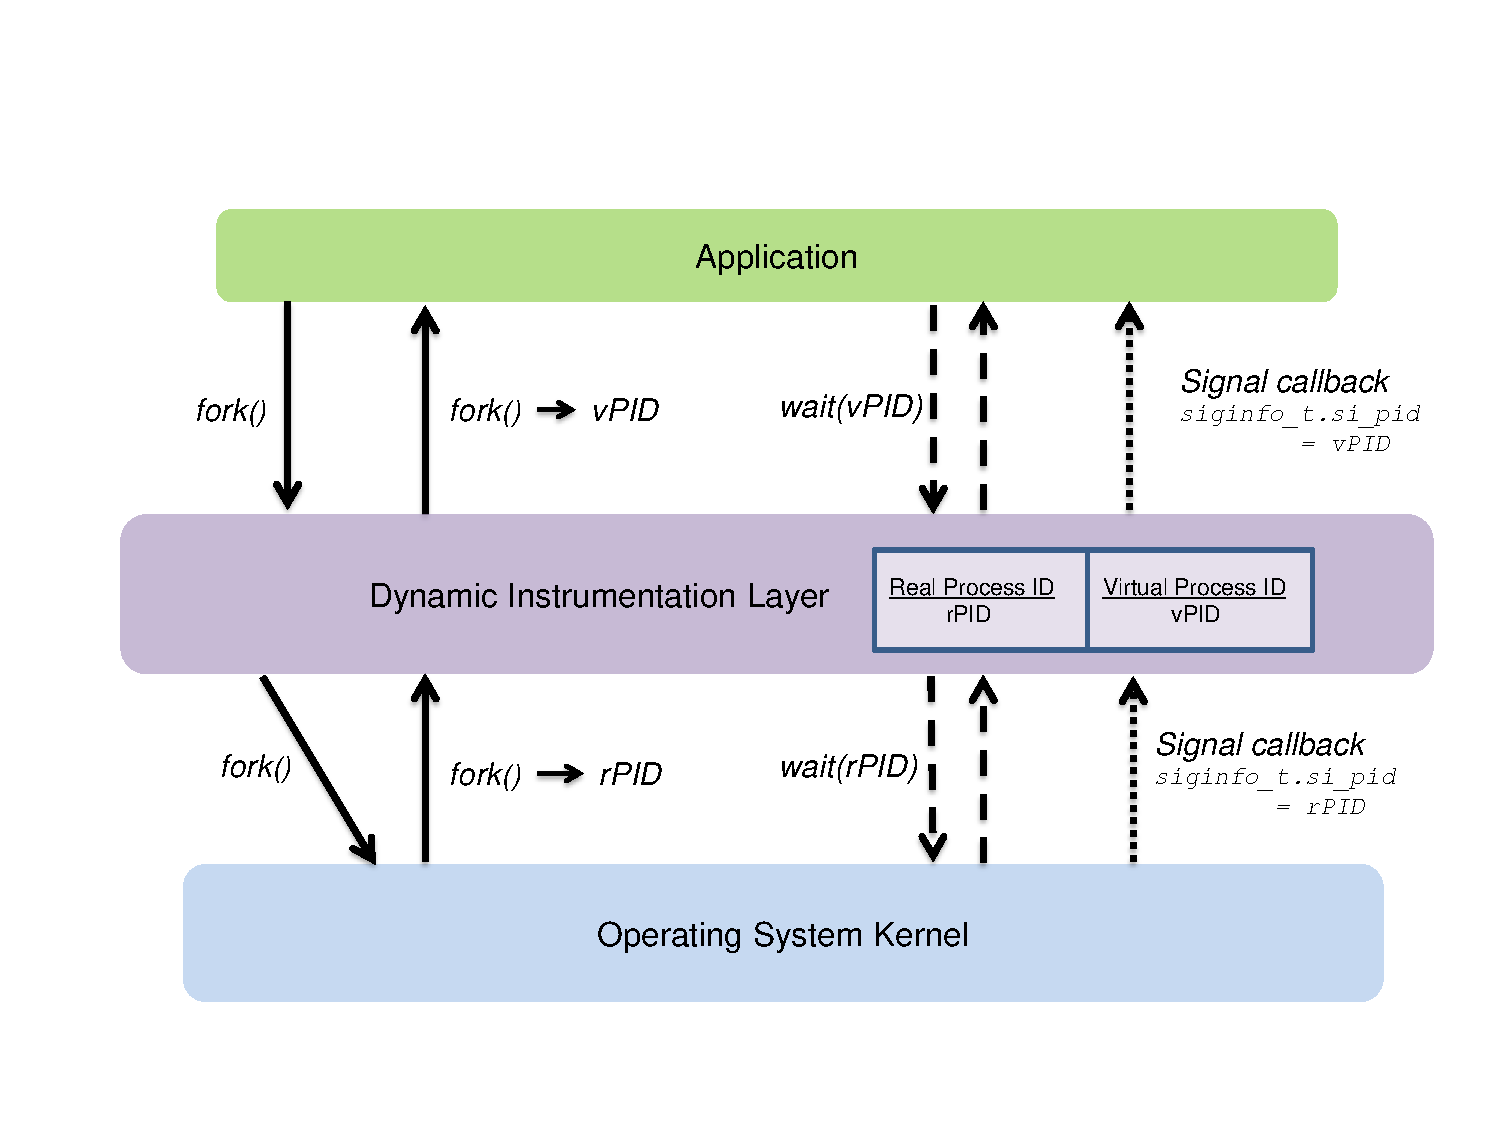
\includegraphics[trim=0cm 1cm 0cm 0.5cm, scale=0.60]{pid.pdf}
  \caption[Virtualizing the process ID layer using Pin]% 
  {All system calls and communications
  between the Linux user and kernel space are intercepted; 
  the dynamic instrumentation layer
  uses a PID translation table, and
  translates between real and virtual process IDs
  to ensure correctness. }
  
  \label{ch3:pidfig}
\end{figure} 

Using dynamic instrumentation, we can replace
real and unpredictable process IDs from kernel space
with virtual and unpredictable process IDs in user space.
As outlined in Section \ref{ch3:pid}, all interfaces
which use process IDs need to be carefully monitored
so that process IDs can be translated back and forth
for correctness. \newline

\noindent {\bf File I/O} \newline
Differences in input file contents across
executions would inevitably cause execution
to diverge, but overcoming nondeterminism arising
from time, randomization or process ID system calls
is typically sufficient to ensure that
file contents rarely differ in Linux services,
if at all. Some files that may differ
between two instances on start up (e.g. 
cache files or logs) can simply be 
deleted or replaced without sacrificing correctness.
Also, as mentioned already, \texttt{stat} 
timestamps are frequently not read, so
they can be replaced with fixed constants;
when they are read and only compared with other
\texttt{stat} timestamps, they can be replaced with 
ordinal numbers that perserve ordering;  
in all other cases, \texttt{stat} system calls 
can be faithfully replayed. \newline

\noindent{\bf Network I/O} \newline
The content of network configuration files
does not change in our experiments, so the strategies 
described to handle \texttt{stat} timestamps 
are sufficient for them. In the same vein, whenever an address is resolved
differently between execution instances because of DNS-based dynamic load balancing, 
we can intercept and replace resolved IPs with those
stored in the execution signature file.

If bytes read from sockets differ across different executions,
we need to understand the {\em context} to determine whether the
differences are serious (e.g. due to different requests)
or synthetic (e.g. due to timestamps). This can
can complicate design of the dynaminc instrumentation
layer because it 
may have to re-execute application or \texttt{libc}
logic to understand differences in raw bytes read from system calls.
We handle nondeterminism from \texttt{Netlink}
sockets in this way: the dynamic instrumentation layer 
re-executes \texttt{libc} logic associated
with understanding contents of \texttt{RTM\_NEWLINK}
messages to detect nondeterminsm from source/destination 
IDs, sequence numbers or interface statistics.
To handle variability in interface statistics,
we can simply overwrite them with fixed values.
This scheme can be generalized to handle
other kinds of network protocols as well.

As an alternative, we could
aggressively intercept Linux socket calls
and blindly replay them in all followers.
When many concurrent executions are reading data from the
same network source, this simulates the possibility
that all instances see the same results over the network
as the first instance. Such an approach, however,
can break correctness (Section \ref{ch3:issues}).
          
\newpage 
To overcome nondeterminism from ephemeral ports, 
we monitor the \texttt{bind} or \texttt{connect} 
system calls and change their arguments to explicitly request ports
in the ephemeral range rather than let the kernel 
assign them; if necessary,
we can also virtualize ephemeral ports
in a similar fashion to how we virtualize process IDs. \newline


\noindent{\bf Scalable I/O Schemes} \newline
To handle nondeterminism caused by unpredictable
ordering of I/O events,
we use techniques similar to those used 
for reordering signals,
as described by Figure \ref{ch3:reorderfig}.

\begin{figure}[h]
  \center
  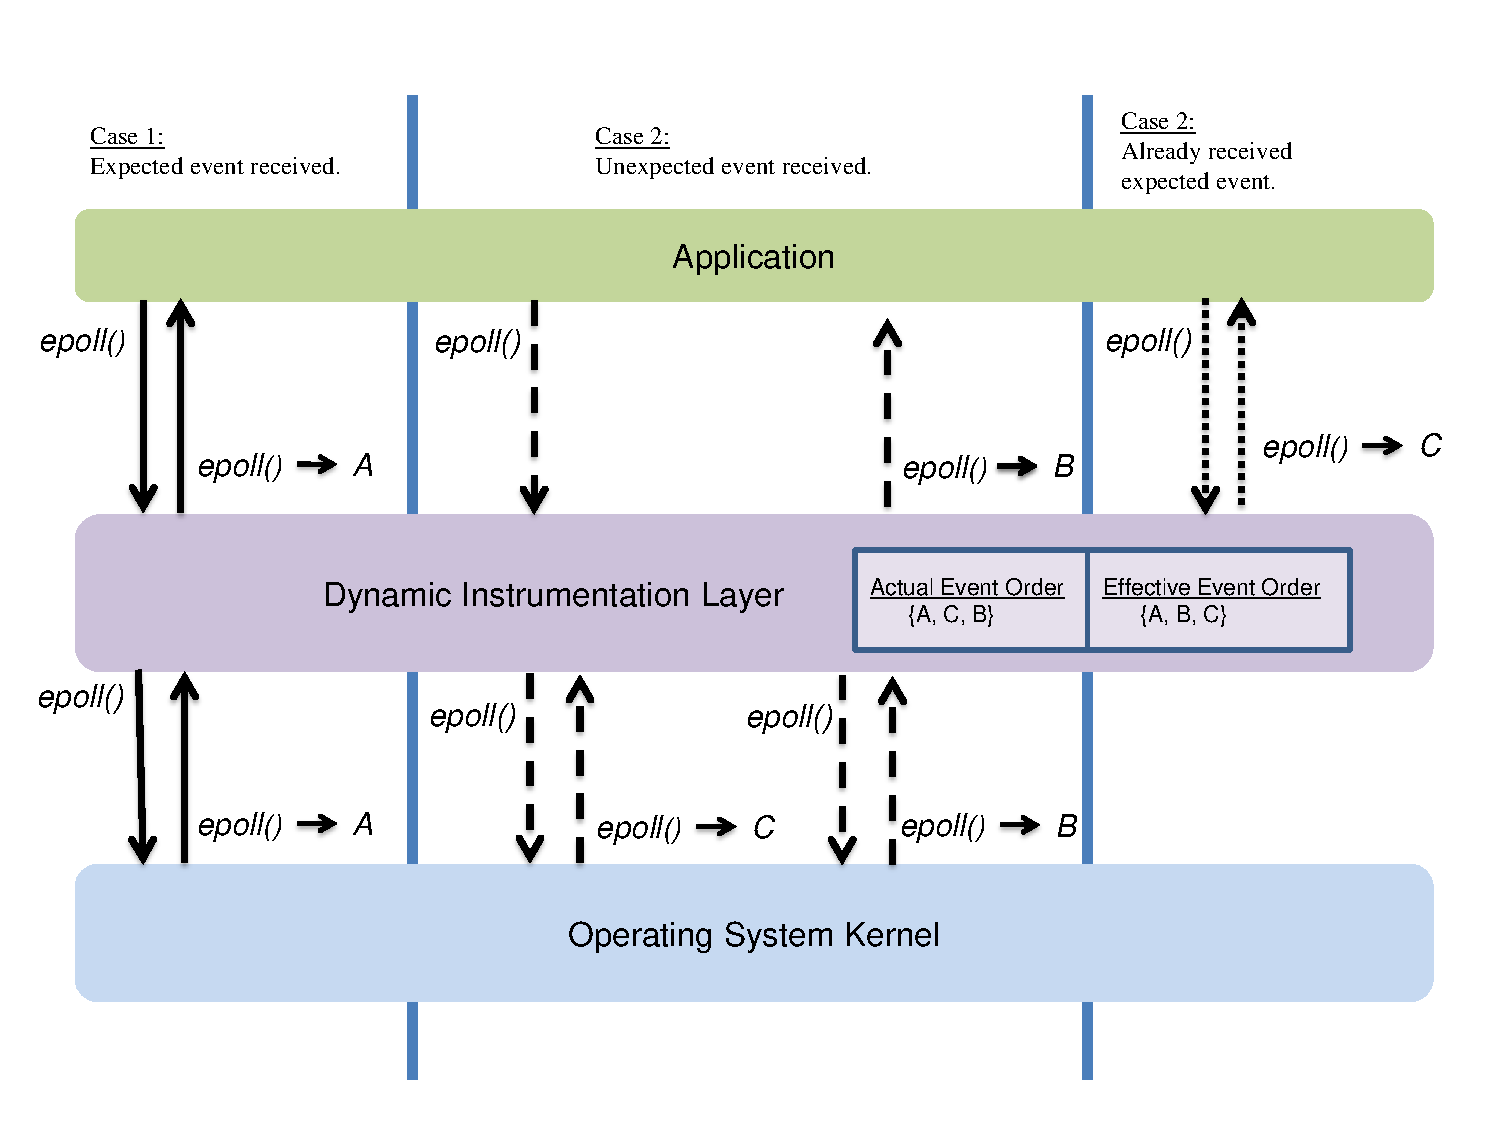
\includegraphics[trim=0cm 1.25cm 0cm 0.75cm, scale=0.60]{epoll.pdf}
  \caption[Reordering I/O events using Pin]% 
    {We intercept all \texttt{epoll} system calls,
    and use the execution signature file to
    achieve determinism. We do not ``replay'' I/O
    events because only events that actually do occur
    are delivered to the application instance. This
    diagram assumes \texttt{epoll} returns one event
    per call for the sake of illustration. }       
  \label{ch3:reorderfig}
\end{figure} 
              
Assuming that \texttt{epoll} returns just one event, figure
\ref{ch3:reorderfig} illustrates three possible cases that could occur:
\begin{itemize}
    \item The event returned by a call to \texttt{epoll} ($A$) is the one expected
    in the execution signature file ($A$). The instrumentation layer
    does not modify the system call.
    \item The desired event ($B$) has not been received yet,
    and \texttt{epoll} returns an unexpected event ($C$).
    The instrumentation layer stores the out-of-order event,
    and repeatedly calls \texttt{epoll} until the 
    the expected event is received.
    \item  A call to \texttt{epoll} is initiated, and the
    event desired ($C$) has already been received.
    The instrumentation layer does not 
    make a system call and simulates a return
    from \texttt{epoll} with the expected event instead.
\end{itemize}

Even if I/O events are reordered,
it is possible that different amounts
of data are available for ready
file descriptors across executions. We can 
mask this effect in the same
way we handle signals: if more bytes
are available (e.g. through \texttt{read}) 
than expected in the execution signature
file, we modify return values and \texttt{read}
buffers to delay the reading of these bytes
until the next \texttt{read}. In some corner
cases, we may have to ``fake'' readiness
in a call to \texttt{epoll}: if all bytes to be read from
a file descriptor have been read by 
the dynamic instrumentation layer (out of which
a few have not yet been delivered to the application),
there will be no more readiness events even
though the application expects them. If less-than-expected
bytes are available, we simply wait
till they are available by waiting for
another readiness update on the same file descriptor inside 
dynamic instrumentation layer.
In our experiments, this approach has been sufficient 
for overcoming nondeterminsm from event-based I/O
schemes.

For asynchronous I/O schemes (e.g. \texttt{aio\_read}), strategies
similar to those used for reordering
and precisely-timing signals would be necessary to hide
variable I/O latency and ordering.
\newline

\noindent {\bf Concurrency} \newline
Nondeterminism due to multi-threading
has been extensively documented; there
is a significant body of work that
attempts to overcome such nondeterminism
by using deterministic logical clocks
or record-and-replay approaches. 
For our experiments, we did not attempt to enforce
a total order on the instructions executed in multi-threaded
programs and just measured nondeterminism inside 
the main process for each Linux service.
To overcome nondeterminism caused
by multi-threading, we could incorporate
deterministic logical clocks 
into our design by augmenting the
execution signature file.

As mentioned before, a nondeterministic system scheduler
can cause variable timing of signals
or I/O events, which
can be handled using reordering and
timing strategies.
Work on deterministic
operating systems can
be extended to overcome this issue
in a more systematic manner. \newline

\noindent {\bf {\em Procfs}: The \texttt{`/proc/directory'}} \newline
Using the techniques described
already, I/O operations on {\em procfs} can be intercepted
and modified. We can 
replay reads from {\em procfs} using the execution signature
file if necessary or replace any statistics with fixed and 
reasonable values. The dynamic instrumentation layer 
must respect differences in virtual and real processes:
it must modify all \texttt{open} system calls with paths
of the form \texttt{`proc/[PID]'}
by switching real and virtual process IDs,
and a process must see its 
parent's virtual process ID when it reads
\texttt{`/proc/[PID]/status'}.

%\section{Results after Using Deterministic Execution} \label{ch3:data}
%We were able to achieve {\em fully} deterministic execution (i.e.
%user-mode execution traces that were 100\% identical) in several
%Linux services including \texttt{cron}, \texttt{ntp} and
%\texttt{cups} using these approaches.

%The next chapter describes the context in which nondeterminism
%occured in these services and the relative
%signficance of the various factors we have outline 
%as sources of nondeterminism in programs.








\section{Evaluation of Simulation} \label{sileval}
In order to evaluate the feasibility of this design,
we need to 
\section {Summary}
